\documentclass[12pt,a4paper,oneside]{book}

\usepackage[utf8]{inputenc}
\usepackage[T1]{fontenc}
\usepackage{lmodern}
\usepackage{graphicx}
\usepackage{amsmath,amssymb}
\usepackage{geometry}
\usepackage{hyperref}
\usepackage{xcolor}
\usepackage{listings}
\usepackage{microtype}

\geometry{margin=1in}

\makeatletter
\newcommand{\chapterauthor}[1]{%
  {\parindent0pt\vspace*{-15pt}%
  \linespread{1.1}\large\itshape\begin{flushright}#1\end{flushright}%
  \par\nobreak\vspace*{25pt}}
  \@afterheading%
}
\makeatother

\begin{document}

\mainmatter

% =====================================================================
% C++ OOP Mini-Project Chapter
% File: XX_CodeAgent.tex  (replace XX with the assigned project number)
% =====================================================================

% ---------- Chapter-local helpers (only standard packages are used) ----------
\lstdefinestyle{codeagentcpp}{
  language=C++,
  basicstyle=\ttfamily\footnotesize,
  keywordstyle=\color{blue!70!black}\bfseries,
  commentstyle=\color{green!45!black}\itshape,
  stringstyle=\color{red!60!black},
  numbers=left, numberstyle=\tiny\color{gray}, numbersep=6pt,
  frame=single, rulecolor=\color{gray!60},
  breaklines=true, breakatwhitespace=false,
  showstringspaces=false, tabsize=4, columns=fullflexible,
  captionpos=b, upquote=true
}
\lstdefinestyle{codeagentplain}{
  basicstyle=\ttfamily\footnotesize,
  frame=single, rulecolor=\color{gray!60},
  breaklines=true, showstringspaces=false, columns=fullflexible,
  captionpos=b, upquote=true
}
% Inserts a screenshot if the file exists; otherwise draws a labelled
% placeholder box so the chapter always compiles.
\newcommand{\codeagentShot}[3][0.6]{%
  \IfFileExists{#2}%
    {\includegraphics[width=0.95\linewidth,height=#1\textheight,keepaspectratio]{#2}}%
    {\fbox{\parbox[c][4.5cm][c]{0.9\linewidth}{\centering\small
      \textbf{Screenshot placeholder}\\[4pt] \texttt{#2}\\[4pt] #3}}}%
}
% Float placement for this chapter: fewer half-empty float pages. The
% previous values are restored at the end of the chapter.
\let\codeagentOldTopfraction\topfraction
\let\codeagentOldBottomfraction\bottomfraction
\let\codeagentOldTextfraction\textfraction
\let\codeagentOldFloatpagefraction\floatpagefraction
\edef\codeagentOldTopnumber{\the\value{topnumber}}
\edef\codeagentOldTotalnumber{\the\value{totalnumber}}
\renewcommand{\topfraction}{0.9}
\renewcommand{\bottomfraction}{0.8}
\renewcommand{\textfraction}{0.07}
\renewcommand{\floatpagefraction}{0.8}
\setcounter{topnumber}{3}
\setcounter{totalnumber}{5}

\chapter[CodeAgent: An LLM-Powered C++ Coding Copilot]{CodeAgent: An LLM-Powered C++ Coding Copilot with CLI and Browser GUI}
\chapterauthor{Lalitadithya Kariyam (251130) \\ Samuel John (251118)}

% =====================================================================
\section{Introduction and Problem Statement}
% =====================================================================

Large language models (LLMs) can write and improve source code, but using them
from a chat website is awkward for real development work. The developer has to:
\begin{itemize}
  \item copy code in and out by hand;
  \item check whether the answer is complete;
  \item avoid pasting secrets such as API keys;
  \item make sure nothing overwrites their files by accident.
\end{itemize}
There is no review step between \emph{``the model suggested a change''} and
\emph{``my file was changed''}.

\textbf{CodeAgent} solves this. It is a C++17 application that connects
Google's Gemini model to a developer's local workflow through two front ends
that share one backend:

\begin{enumerate}
  \item \textbf{A command-line interface (CLI):}
    \begin{itemize}
      \item \texttt{codeagent generate "<instruction>"} generates code and
        offers to save it.
      \item \texttt{codeagent refactor <file> "<instruction>"} reads a file,
        asks Gemini for an improved version, shows a unified diff, and writes
        the file only after explicit approval.
    \end{itemize}
  \item \textbf{A browser-based GUI} (\texttt{codeagent gui}). The same
    executable starts a local, loopback-only HTTP server. That server serves
    an editor page and a JSON API offering generation, refactoring proposals,
    diff review, approve and reject, and safe file saving.
\end{enumerate}

\subsection*{End-user view}
The user types an instruction in plain English, either in the terminal or in
the browser chat panel. CodeAgent builds a carefully worded prompt, sends it
over HTTPS to Gemini, checks that the reply is complete and usable, and
displays the code. For a refactoring, the user always sees what will change
before anything happens.

\subsection*{Software requirements}
\begin{itemize}
  \item[\textbf{R1}] Generate code from a natural-language instruction.
  \item[\textbf{R2}] Refactor an existing text file and present the change as
    a diff.
  \item[\textbf{R3}] Never modify a file without explicit user consent;
    approval and saving are separate actions.
  \item[\textbf{R4}] Read and write files safely: atomic replacement, no
    silent overwrite, no symbolic-link targets, and no secret
    (\texttt{.env}) files.
  \item[\textbf{R5}] Keep the API key secret: never in a URL, never in logs,
    never sent to the browser.
  \item[\textbf{R6}] Report every failure (network, quota, invalid key,
    blocked or incomplete response, file error) with a clear, actionable
    message instead of crashing.
  \item[\textbf{R7}] Offer the same core features from both a CLI and a GUI
    without duplicating backend logic.
  \item[\textbf{R8}] Be testable without network access or a real Gemini
    account.
\end{itemize}

% =====================================================================
\section{Scope and Feature Set}
% =====================================================================

\begin{itemize}
  \item \textbf{AI code generation (CLI and GUI):} instruction + language
    $\rightarrow$ Gemini $\rightarrow$ validated source code. In the CLI the
    result can be saved to a user-chosen path. In the GUI it is accepted into
    the editor and then saved with \emph{Save As}.
  \item \textbf{AI refactoring with review:} the CLI shows a unified diff and
    asks \texttt{Apply these changes? [y/\allowbreak{}N]}. The GUI creates a server-side
    \emph{proposal} (\texttt{PENDING}) that must be reviewed as a diff, then
    approved or rejected. Approval only updates the editor; saving is a
    separate, explicit step.
  \item \textbf{Safe file I/O and persistent storage:} UTF-8 text files of
    any extension are read and written atomically (temporary file + rename);
    binary content and environment (\texttt{.env}) files are refused;
    overwriting needs confirmation; external modification is detected with a
    content revision hash; ``always allow'' permissions persist in
    \texttt{.codeagent/\allowbreak{}\allowbreak permissions.txt}; configuration comes
    from layered \texttt{.env} files.
  \item \textbf{Robust Gemini integration:} HTTPS through libcurl with TLS
    verification, timeouts and a 2\,MiB response limit; strict JSON
    validation; finish-reason checking (a refactoring must be explicitly
    complete); removal of Markdown code fences; optional display of the
    model's ``thoughts''.
  \item \textbf{Typed error handling:} a polymorphic exception hierarchy maps
    each failure to a user message, a machine-readable code and an HTTP
    status, with automatic secret redaction.
  \item \textbf{Secure local web server:} bound to \texttt{127.0.0.1}
    only, with a one-time bootstrap code exchanged for a 256-bit session
    token, Host and Origin header checks, a strict Content Security Policy, a
    1\,MiB request limit and exact-shape JSON validation.
  \item \textbf{Native dialogs:} OS file and folder pickers (zenity on Linux;
    a Windows dialog through PowerShell under WSL), started without a shell.
  \item \textbf{Automated tests:} 214 GoogleTest cases (C++) and 79 Node.js
    tests (frontend), none of which need the internet.
\end{itemize}

\subsection*{Out of scope (current limitations)}
\begin{itemize}
  \item Linux and WSL2 are the supported platforms; native Windows and macOS
    builds were not verified.
  \item The GUI editor is a plain text area (no syntax highlighting).
  \item Proposals are kept in memory and are lost when the server stops.
  \item Generated code is not compiled or executed by CodeAgent.
  \item The CLI \texttt{generate} command always targets C++; the GUI lets
    the user choose the language.
\end{itemize}

% =====================================================================
\section{Evaluation Criteria Mapping}
% =====================================================================

Table~\ref{tab:ca-rubric} shows where each evaluation criterion is addressed
in this report and in the repository.

\begin{table}[htbp]
\centering\small
\begin{tabular}{|p{3.2cm}|p{5.3cm}|p{5.5cm}|}
\hline
\textbf{Criterion} & \textbf{Report sections} & \textbf{Repository evidence} \\ \hline
OOP Architecture \& Design (25) &
\ref{sec:ca-oop} Object-Oriented Architecture, \ref{sec:ca-uml} UML &
\texttt{include/\allowbreak{}*.hpp}, \texttt{UML-diagrams.md} \\ \hline
Advanced C++ Mechanics (20) &
\ref{sec:ca-adv} Advanced C++ Mechanics &
\texttt{CodeAgentError.*}, \texttt{LLMClient.cpp}, \texttt{FileManager.cpp}, \texttt{GuiHttpServer.cpp} \\ \hline
Frontend \& Backend Integration (20) &
\ref{sec:ca-tech} Technology Stack, \ref{sec:ca-integration} Integration, \ref{sec:ca-storage} Persistent Storage &
\texttt{src/\allowbreak{}}, \texttt{frontend/\allowbreak{}}, \texttt{docs/\allowbreak{}gui-api-contract.md} \\ \hline
Version Control (10) &
\ref{sec:ca-git} Version Control &
61 commits, 6 branches, 3 merge commits \\ \hline
Documentation \& Analysis (10) &
This chapter, \ref{sec:ca-testing} Testing &
\texttt{README.md}, \texttt{docs/\allowbreak{}} \\ \hline
Demonstration \& Viva (15) &
\ref{sec:ca-results} Results, \ref{sec:ca-demo} Demo plan &
\texttt{docs/\allowbreak{}demo-and-viva.md}, \texttt{scripts/\allowbreak{}smoke-test.sh} \\ \hline
\end{tabular}
\caption{Evaluation criteria and supporting evidence}
\label{tab:ca-rubric}
\end{table}

% =====================================================================
\section{Technology Stack}
\label{sec:ca-tech}
% =====================================================================

Table~\ref{tab:ca-tech} lists the technologies used in each layer of
CodeAgent. All business logic is written in C++; the browser frontend uses
plain web technologies with no framework or build step.

\begin{table}[htbp]
\centering\small
\begin{tabular}{|p{2.8cm}|p{5.2cm}|p{6.0cm}|}
\hline
\textbf{Layer} & \textbf{Technology} & \textbf{Used for} \\ \hline
Language & C++17 & All backend logic and the CLI \\ \hline
Build & CMake 3.15+, FetchContent & Libraries, the executable and test targets \\ \hline
AI model & Google Gemini API & Code generation and refactoring \\ \hline
HTTP client & libcurl (HTTPS, TLS verification) & Outbound requests to Gemini \\ \hline
JSON & nlohmann/json & Gemini requests and responses, API payloads \\ \hline
HTTP server & cpp-httplib 0.58 & Local JSON API on \texttt{127.0.0.1} \\ \hline
Frontend & HTML, CSS, JavaScript (ES modules) & Editor, chat and diff review in the browser \\ \hline
Testing & GoogleTest 1.14 with CTest; \texttt{node:test} & 214 C++ tests and 79 frontend tests \\ \hline
Platform & Linux / WSL2; zenity or PowerShell & Runtime and native file dialogs \\ \hline
Version control & Git and GitHub & Feature branches, 61 commits by both members \\ \hline
\end{tabular}
\caption{Technology stack}
\label{tab:ca-tech}
\end{table}

\paragraph{Why these choices.}
\begin{itemize}
  \item \textbf{C++17} provides \texttt{std::filesystem}, \texttt{std::optional}
    and the object-oriented features the project is built on, and keeps the
    API key and all file access inside the native process.
  \item \textbf{libcurl and cpp-httplib play opposite roles}: libcurl is the
    client that sends requests out to Gemini, while cpp-httplib is the server
    that receives requests from the browser.
  \item \textbf{No frontend framework}: the C++ executable serves the static
    HTML, CSS and JavaScript files itself, so the GUI needs no separate
    process or build tool.
  \item \textbf{Pinned dependencies}: GoogleTest v1.14.0 and cpp-httplib
    v0.58.0 are fetched at fixed versions, so every build uses the same code.
\end{itemize}

% =====================================================================
\section{System Architecture Overview}
% =====================================================================

CodeAgent is a \textbf{single executable} built in three layers:

\begin{description}
  \item[Presentation layer (front ends).]
    \texttt{CLIController} (terminal) and the browser application in
    \texttt{frontend/\allowbreak{}} (HTML, CSS and ES-module JavaScript). The browser never
    talks to Gemini and never touches the disk; it only calls the local API.
  \item[Application / service layer.]
    \texttt{GuiHttpServer} exposes the backend over HTTP and owns proposal
    state. It does \emph{not} call Gemini itself: it receives
    \emph{generation} and \emph{refactoring handlers} (function objects) from
    \texttt{CLIController}, so the Gemini logic exists only once.
  \item[Core / domain layer.]
    \texttt{PromptBuilder} (prompt text), \texttt{LLMClient} (HTTPS to
    Gemini), \texttt{ResponseParser} (JSON interpretation),
    \texttt{FileManager} (CLI file I/O with consent), \texttt{makeUnifiedDiff}
    (line diff), \texttt{EnvLoader} (configuration), \texttt{CodeAgentError}
    (failure model) and \texttt{NativeDialog\allowbreak{}Provider} (OS dialogs).
\end{description}

\begin{lstlisting}[style=codeagentplain,caption={Layered architecture of CodeAgent},label={lst:ca-arch}]
 Terminal user                          Browser user (frontend/js/app.js, api.js)
      |                                        |  HTTP + JSON + X-CodeAgent-Token
      v                                        v  127.0.0.1:8080
 main.cpp -> CLIController  --- "gui" --->  GuiHttpServer (cpp-httplib, pimpl)
      |   |   |                                |   |   |
      |   |   +--> FileManager (terminal)      |   |   +--> NativeDialogProvider
      |   +------> makeUnifiedDiff <-----------+   +------> GUI safe file I/O
      |                                        |
      +--> PromptBuilder <-- handlers ---------+
               |
               v
           LLMClient --> ResponseParser
               |  (EnvLoader: GEMINI_API_KEY)
               v  HTTPS (libcurl)
           Google Gemini API
\end{lstlisting}

% =====================================================================
\section{Object-Oriented Architecture}
\label{sec:ca-oop}
% =====================================================================

The design applies the core OOP principles throughout: each class has a single
responsibility, data is hidden behind small public interfaces, related
failures are modelled by inheritance, behaviour varies through virtual
functions, and objects are composed and injected rather than hard-wired.

\subsection{Class Design and Associations}

Table~\ref{tab:ca-classes} lists the primary classes and the responsibility of
each.

\begin{table}[htbp]
\centering\small
\begin{tabular}{|p{3.6cm}|p{6.2cm}|p{4.2cm}|}
\hline
\textbf{Class} & \textbf{Responsibility} & \textbf{Files} \\ \hline
\texttt{CLIController} & Parses commands, runs the CLI workflows, starts the GUI, and is the CLI error boundary & \texttt{CLIController.hpp/\allowbreak{}.cpp} \\ \hline
\texttt{PromptBuilder} & Builds deterministic generation and refactoring prompts; validates inputs & \texttt{PromptBuilder.hpp/\allowbreak{}.cpp} \\ \hline
\texttt{LLMClient} & Sends prompts to Gemini over HTTPS; maps failures to typed exceptions & \texttt{LLMClient.hpp/\allowbreak{}.cpp} \\ \hline
\texttt{ResponseParser} & Validates Gemini JSON and extracts text and thoughts; classifies finish reasons & \texttt{ResponseParser.hpp/\allowbreak{}.cpp} \\ \hline
\texttt{FileManager} & Terminal-mediated reading and writing with permission prompts and atomic writes & \texttt{FileManager.hpp/\allowbreak{}.cpp} \\ \hline
\texttt{GuiHttpServer} (+ \texttt{Impl}) & Local HTTP API, session security, proposal store, GUI file I/O & \texttt{GuiHttpServer.hpp/\allowbreak{}.cpp} \\ \hline
\texttt{NativeDialog\allowbreak{}Provider} (abstract) and \texttt{SystemNative\allowbreak{}DialogProvider} & Interface and implementation for OS file and folder pickers & \texttt{NativeDialog.hpp/\allowbreak{}.cpp} \\ \hline
\texttt{CodeAgentError} (abstract) + 12 subclasses & Typed, safe failure model with \texttt{code()} and \texttt{httpStatus()} & \texttt{CodeAgentError.hpp/\allowbreak{}.cpp} \\ \hline
Data types: \texttt{ParsedResponse}, \texttt{ProviderError\allowbreak{}Details}, \texttt{GenerationResult}, \texttt{NativeDialogResult}, \texttt{PendingProposal} & Plain structures that carry results between classes & various \\ \hline
\end{tabular}
\caption{Primary classes and responsibilities}
\label{tab:ca-classes}
\end{table}

\paragraph{Inheritance.}
\begin{itemize}
  \item A three-level hierarchy of exceptions derives from
    \texttt{std::\allowbreak{}runtime\_error} (Listing~\ref{lst:ca-hier}).
  \item \texttt{SystemNative\allowbreak{}DialogProvider} inherits from (implements) the
    abstract interface \texttt{NativeDialog\allowbreak{}Provider}.
  \item In the tests, \texttt{ScriptedNativeDialogProvider} implements the
    same interface.
\end{itemize}

\begin{lstlisting}[style=codeagentplain,caption={Exception inheritance hierarchy (is-a relationships)},label={lst:ca-hier}]
std::runtime_error
 +-- CodeAgentError                  <<abstract>>  code(), httpStatus() pure virtual
      +-- ConfigurationError         CONFIGURATION_ERROR        503
      +-- ProviderError              PROVIDER_ERROR             502
      |    +-- AuthenticationError   PROVIDER_AUTH_FAILED       502
      |    +-- RateLimitError        PROVIDER_RATE_LIMITED /
      |    |                         PROVIDER_QUOTA_EXHAUSTED   429
      |    +-- ProviderUnavailableError  PROVIDER_UNAVAILABLE   503
      |    +-- NetworkError          PROVIDER_UNREACHABLE       502
      |    |    +-- TimeoutError     PROVIDER_TIMEOUT           504
      |    +-- ProviderResponseError PROVIDER_RESPONSE_*        502
      +-- FileError                  READ_FAILED / SAVE_FAILED  500
           +-- FilePermissionError   PERMISSION_DENIED          403
           +-- FileNotFoundError     FILE_NOT_FOUND             404
           +-- FileConflictError     FILE_CHANGED_ON_DISK       409
\end{lstlisting}

\paragraph{Composition (strong ownership).}
\begin{itemize}
  \item \texttt{GuiHttpServer} \emph{owns} its \texttt{Impl} through
    \texttt{std::\allowbreak{}unique\_ptr<Impl>}.
  \item \texttt{Impl} owns an \texttt{httplib::\allowbreak{}Server}, the listener
    \texttt{std::\allowbreak{}thread}, the proposal map
    (\texttt{std::\allowbreak{}map<std::\allowbreak{}string, PendingProposal>}), the LRU list of opened
    documents, and the session secrets.
\end{itemize}
These parts are created and destroyed together with their owner.

\paragraph{Aggregation (shared, non-owning or shared ownership).}
\begin{itemize}
  \item \texttt{GuiHttpServer} holds a
    \texttt{std::\allowbreak{}shared\_ptr<NativeDialogProvider>} that can be shared with,
    and outlive, the server (a test keeps its own reference).
  \item \texttt{CLIController} and \texttt{FileManager} hold
    \emph{references} to streams (\texttt{std::\allowbreak{}istream\&},
    \texttt{std::\allowbreak{}ostream\&}) that they use but do not own.
\end{itemize}

\paragraph{Association / dependency (uses).}
\begin{itemize}
  \item \texttt{CLIController} creates and uses \texttt{PromptBuilder},
    \texttt{FileManager} and \texttt{GuiHttpServer}.
  \item \texttt{LLMClient} uses \texttt{ResponseParser} and
    \texttt{EnvLoader}.
  \item \texttt{GuiHttpServer} uses \texttt{makeUnifiedDiff} and
    \texttt{CodeAgentError}.
\end{itemize}

\subsection{Encapsulation and Access Modifiers}

Every class exposes the smallest useful public interface. Internal steps are
\texttt{private}; constructors meant only for subclasses are
\texttt{protected}. The most important safety rule of the project, \emph{never
overwrite a file without asking}, is enforced by encapsulation: the only public
write paths (\texttt{saveFile}, \texttt{writeFile}) always call the private
\texttt{requestOverwritePermission} before the private
\texttt{writeAtomically}.

\begin{lstlisting}[style=codeagentcpp,caption={Access modifiers in \texttt{FileManager} (abridged)},label={lst:ca-fm}]
class FileManager {
public:
    enum class WriteResult { Written, InvalidPath, Declined, Failed };
    enum class PermissionPrompt { Ask, AlreadyGranted };

    FileManager();
    FileManager(std::istream& input, std::ostream& output, std::ostream& error);

    bool readFile(const std::filesystem::path& filePath, std::string& content) const;
    bool writeFile(const std::filesystem::path& filePath, const std::string& content) const;
    WriteResult saveFile(const std::filesystem::path& filePath, const std::string& content,
                         PermissionPrompt prompt = PermissionPrompt::Ask) const;
    bool isValidSourceFile(const std::filesystem::path& filePath) const;

private:
    enum class PermissionType { Read, Write };
    bool requestPermission(const std::filesystem::path&, PermissionType) const;
    bool requestOverwritePermission(const std::filesystem::path&) const;
    void writeAtomically(const std::filesystem::path&, const std::string&) const;
    bool isSupportedFileName(const std::filesystem::path&) const;

    std::filesystem::path permissionFilePath_;   // .codeagent/permissions.txt
    std::istream& input_;
    std::ostream& output_;
    std::ostream& error_;
};
\end{lstlisting}

\begin{table}[htbp]
\centering\small
\begin{tabular}{|p{3.3cm}|p{4.8cm}|p{5.9cm}|}
\hline
\textbf{Access level} & \textbf{Example} & \textbf{Purpose} \\ \hline
\texttt{public} & \texttt{LLMClient::\allowbreak{}generate}, \texttt{GuiHttpServer::\allowbreak{}start} & Minimal interface used by other modules \\ \hline
\texttt{protected} & \texttt{CodeAgentError(\allowbreak{}userMessage, diagnostic)}, \texttt{NetworkError(msg, diag)} & Only subclasses may construct the abstract base or reuse a constructor \\ \hline
\texttt{private} & \texttt{FileManager::\allowbreak{}writeAtomically}, \texttt{RateLimitError::\allowbreak{}quotaExhausted\_} & Implementation details and invariants \\ \hline
Anonymous \texttt{namespace} & \texttt{performHttpRequest}, \texttt{resolveGuiPort}, \texttt{readRegularFile} & File-private helper functions (encapsulation at translation-unit level) \\ \hline
Pimpl (\texttt{class Impl;}) & \texttt{GuiHttpServer} & Hides all server state and the \texttt{httplib.h} dependency from the public header \\ \hline
\texttt{const} member functions & \texttt{PromptBuilder::\allowbreak{}build\allowbreak{}GenerationPrompt(...) const} & Guarantees that queries do not modify the object \\ \hline
\end{tabular}
\caption{Access control used in the project}
\label{tab:ca-access}
\end{table}

\subsection{Abstraction}
Callers work with simple concepts and never see implementation details:
\begin{itemize}
  \item \texttt{LLMClient::\allowbreak{}generate(prompt, options)} returns text. libcurl,
    HTTP headers, JSON and finish reasons are hidden.
  \item \texttt{makeUnifiedDiff(a, b)} returns a diff. The LCS algorithm
    (Hirschberg) is hidden.
  \item \texttt{NativeDialogProvider::\allowbreak{}choose(kind)} returns a path. Whether
    zenity or PowerShell ran is hidden.
\end{itemize}

\subsection{Polymorphism and Virtual Functions}

\paragraph{Abstract base class with pure virtual functions.}
\texttt{CodeAgentError} declares \texttt{code()} and \texttt{httpStatus()} as
pure virtual, so it cannot be instantiated. Each concrete subclass overrides
them, and \texttt{final} prevents further derivation where that would be
meaningless.

\begin{lstlisting}[style=codeagentcpp,caption={Abstract base class and an overriding subclass},label={lst:ca-virtual}]
class CodeAgentError : public std::runtime_error {
public:
    virtual const char* code() const noexcept = 0;      // pure virtual
    virtual int httpStatus() const noexcept = 0;        // pure virtual
    const std::string& diagnostic() const noexcept;
protected:
    CodeAgentError(const std::string& userMessage, std::string diagnostic);
private:
    std::shared_ptr<const std::string> diagnostic_;     // copying cannot throw
};

class FileNotFoundError final : public FileError {
public:
    FileNotFoundError(FileOperation operation, std::filesystem::path path,
                      std::error_code error);
    const char* code() const noexcept override;         // "FILE_NOT_FOUND"
    int httpStatus() const noexcept override;           // 404
};
\end{lstlisting}

\paragraph{Dynamic dispatch in practice.}
The HTTP server converts \emph{any} error into a JSON response with one
function and no type checks. Adding a new error class requires no change here
(the open/closed principle):

\begin{lstlisting}[style=codeagentcpp,caption={One handler for every error type through virtual calls},label={lst:ca-dispatch}]
void respondWithError(httplib::Response& response, const CodeAgentError& error) {
    logError(std::cerr, error);                       // redacted diagnostic -> terminal
    setJsonError(response, error.httpStatus(),        // virtual: 404, 429, 504, ...
                 error.code(), error.what());         // virtual code, safe message
}
\end{lstlisting}

Catching by base-class reference is polymorphic too.
\texttt{catch (const NetworkError\&)} also catches \texttt{TimeoutError}, and
\texttt{CLIController::\allowbreak{}run} catches every project error with one
\texttt{catch (const CodeAgentError\&)}.

\paragraph{Interface polymorphism.}
\begin{lstlisting}[style=codeagentcpp,caption={Interface with a virtual destructor and two implementations},label={lst:ca-iface}]
class NativeDialogProvider {
public:
    virtual ~NativeDialogProvider() = default;               // safe deletion via base pointer
    virtual NativeDialogResult choose(NativeDialogKind kind) = 0;
};
// Production (src/NativeDialog.cpp): runs zenity / PowerShell without a shell
class SystemNativeDialogProvider final : public NativeDialogProvider {
public:
    NativeDialogResult choose(NativeDialogKind kind) override;
};
// Tests (tests/GuiHttpServerTest.cpp): returns scripted results
class ScriptedNativeDialogProvider final : public NativeDialogProvider { /* ... */ };
\end{lstlisting}

\paragraph{Compile-time polymorphism.}
\begin{itemize}
  \item Function overloading: four \texttt{LLMClient::\allowbreak{}generateContent} and
    \texttt{generateCompleteContent} overloads, and five
    \texttt{GuiHttpServer} constructors.
  \item Template instantiation: see Section~\ref{sec:ca-adv}.
\end{itemize}

\subsection{Dependency Injection and Design Patterns}

Classes receive their collaborators instead of creating them. This makes every
component replaceable and lets all tests run offline (requirement R8).

\begin{table}[htbp]
\centering\small
\begin{tabular}{|p{2.9cm}|p{3.6cm}|p{3.6cm}|p{3.6cm}|}
\hline
\textbf{Class} & \textbf{Injected dependency} & \textbf{Production} & \textbf{Test} \\ \hline
\texttt{LLMClient} & \texttt{HttpTransport} (\texttt{std::\allowbreak{}function}) & libcurl \texttt{performHttpRequest} & lambda returning canned JSON \\ \hline
\texttt{CLIController} & \texttt{LLMCall}, streams, \texttt{GuiCommand} & \texttt{LLMClient}, \texttt{cin}/\texttt{cout}/\texttt{cerr} & fake LLM, string streams \\ \hline
\texttt{GuiHttpServer} & handlers, \texttt{NativeDialog\allowbreak{}Provider}, clock & lambdas calling the core, zenity provider, \texttt{steady\_clock} & fakes, scripted provider, fake clock \\ \hline
\texttt{FileManager} & streams & terminal & string streams \\ \hline
\end{tabular}
\caption{Dependency injection points}
\label{tab:ca-di}
\end{table}

Design patterns used:
\begin{description}
  \item[Pimpl] \texttt{GuiHttpServer::\allowbreak{}Impl}.
  \item[Strategy] Injected \texttt{std::\allowbreak{}function} objects and the dialog
    provider.
  \item[Factory] \texttt{createNativeDialogProvider()} and the named
    constructor \texttt{ConfigurationError::\allowbreak{}missingSetting()}.
  \item[RAII / scope guard] See Section~\ref{sec:ca-adv}.
  \item[Facade] \texttt{LLMClient::\allowbreak{}generate}.
  \item[State machine] Proposal status, on the server and in
    \texttt{proposalWorkflow.js}.
  \item[Composition root] \texttt{runGuiCommand} wires the real
    implementations together.
  \item[LRU cache] \texttt{std::\allowbreak{}list} plus a \texttt{std::\allowbreak{}map} of iterators
    for the documents opened in a session.
\end{description}

% =====================================================================
\section{UML Diagrams}
\label{sec:ca-uml}
% =====================================================================

The repository file \texttt{UML-diagrams.md} contains the complete Mermaid
sources, kept consistent with the code. The class diagram is split into two
views (application classes, Figure~\ref{fig:ca-uml-class}, and the error
hierarchy, Figure~\ref{fig:ca-uml-errors}), followed by three sequence
diagrams and the proposal state diagram.
In the class diagrams, \texttt{+} marks public and \texttt{-} private
members, \texttt{*} marks a pure virtual function, and the stereotypes
\texttt{<{}<abstract>>} and \texttt{<{}<interface>>} mark classes that cannot be
instantiated.

\begin{table}[htbp]
\centering\small
\begin{tabular}{|p{3.6cm}|p{2.6cm}|p{3.6cm}|p{4.0cm}|}
\hline
\textbf{From} & \textbf{Relationship} & \textbf{To} & \textbf{Meaning} \\ \hline
CodeAgentError subclasses & Generalisation & CodeAgentError & is-a (inheritance) \\ \hline
SystemNative\allowbreak DialogProvider & Realisation & NativeDialogProvider & implements the interface \\ \hline
GuiHttpServer & Composition & Impl & owns (\texttt{unique\_ptr}) \\ \hline
GuiHttpServer::Impl & Aggregation & NativeDialogProvider & shares (\texttt{shared\_ptr}) \\ \hline
CLIController & Dependency & PromptBuilder, FileManager, LLMClient, GuiHttpServer & creates and uses \\ \hline
LLMClient & Dependency & ResponseParser, EnvLoader & uses \\ \hline
GuiHttpServer & Dependency & makeUnifiedDiff, CodeAgentError & uses \\ \hline
\end{tabular}
\caption{UML relationships between classes}
\label{tab:ca-uml-rel}
\end{table}

\begin{figure}[htbp]
\centering
% The diagram is much wider than tall, so it is allowed to extend into the
% side margins (nearly the full paper width), centred on the page.
\IfFileExists{screenshots/uml-class.png}%
  {\makebox[\linewidth][c]{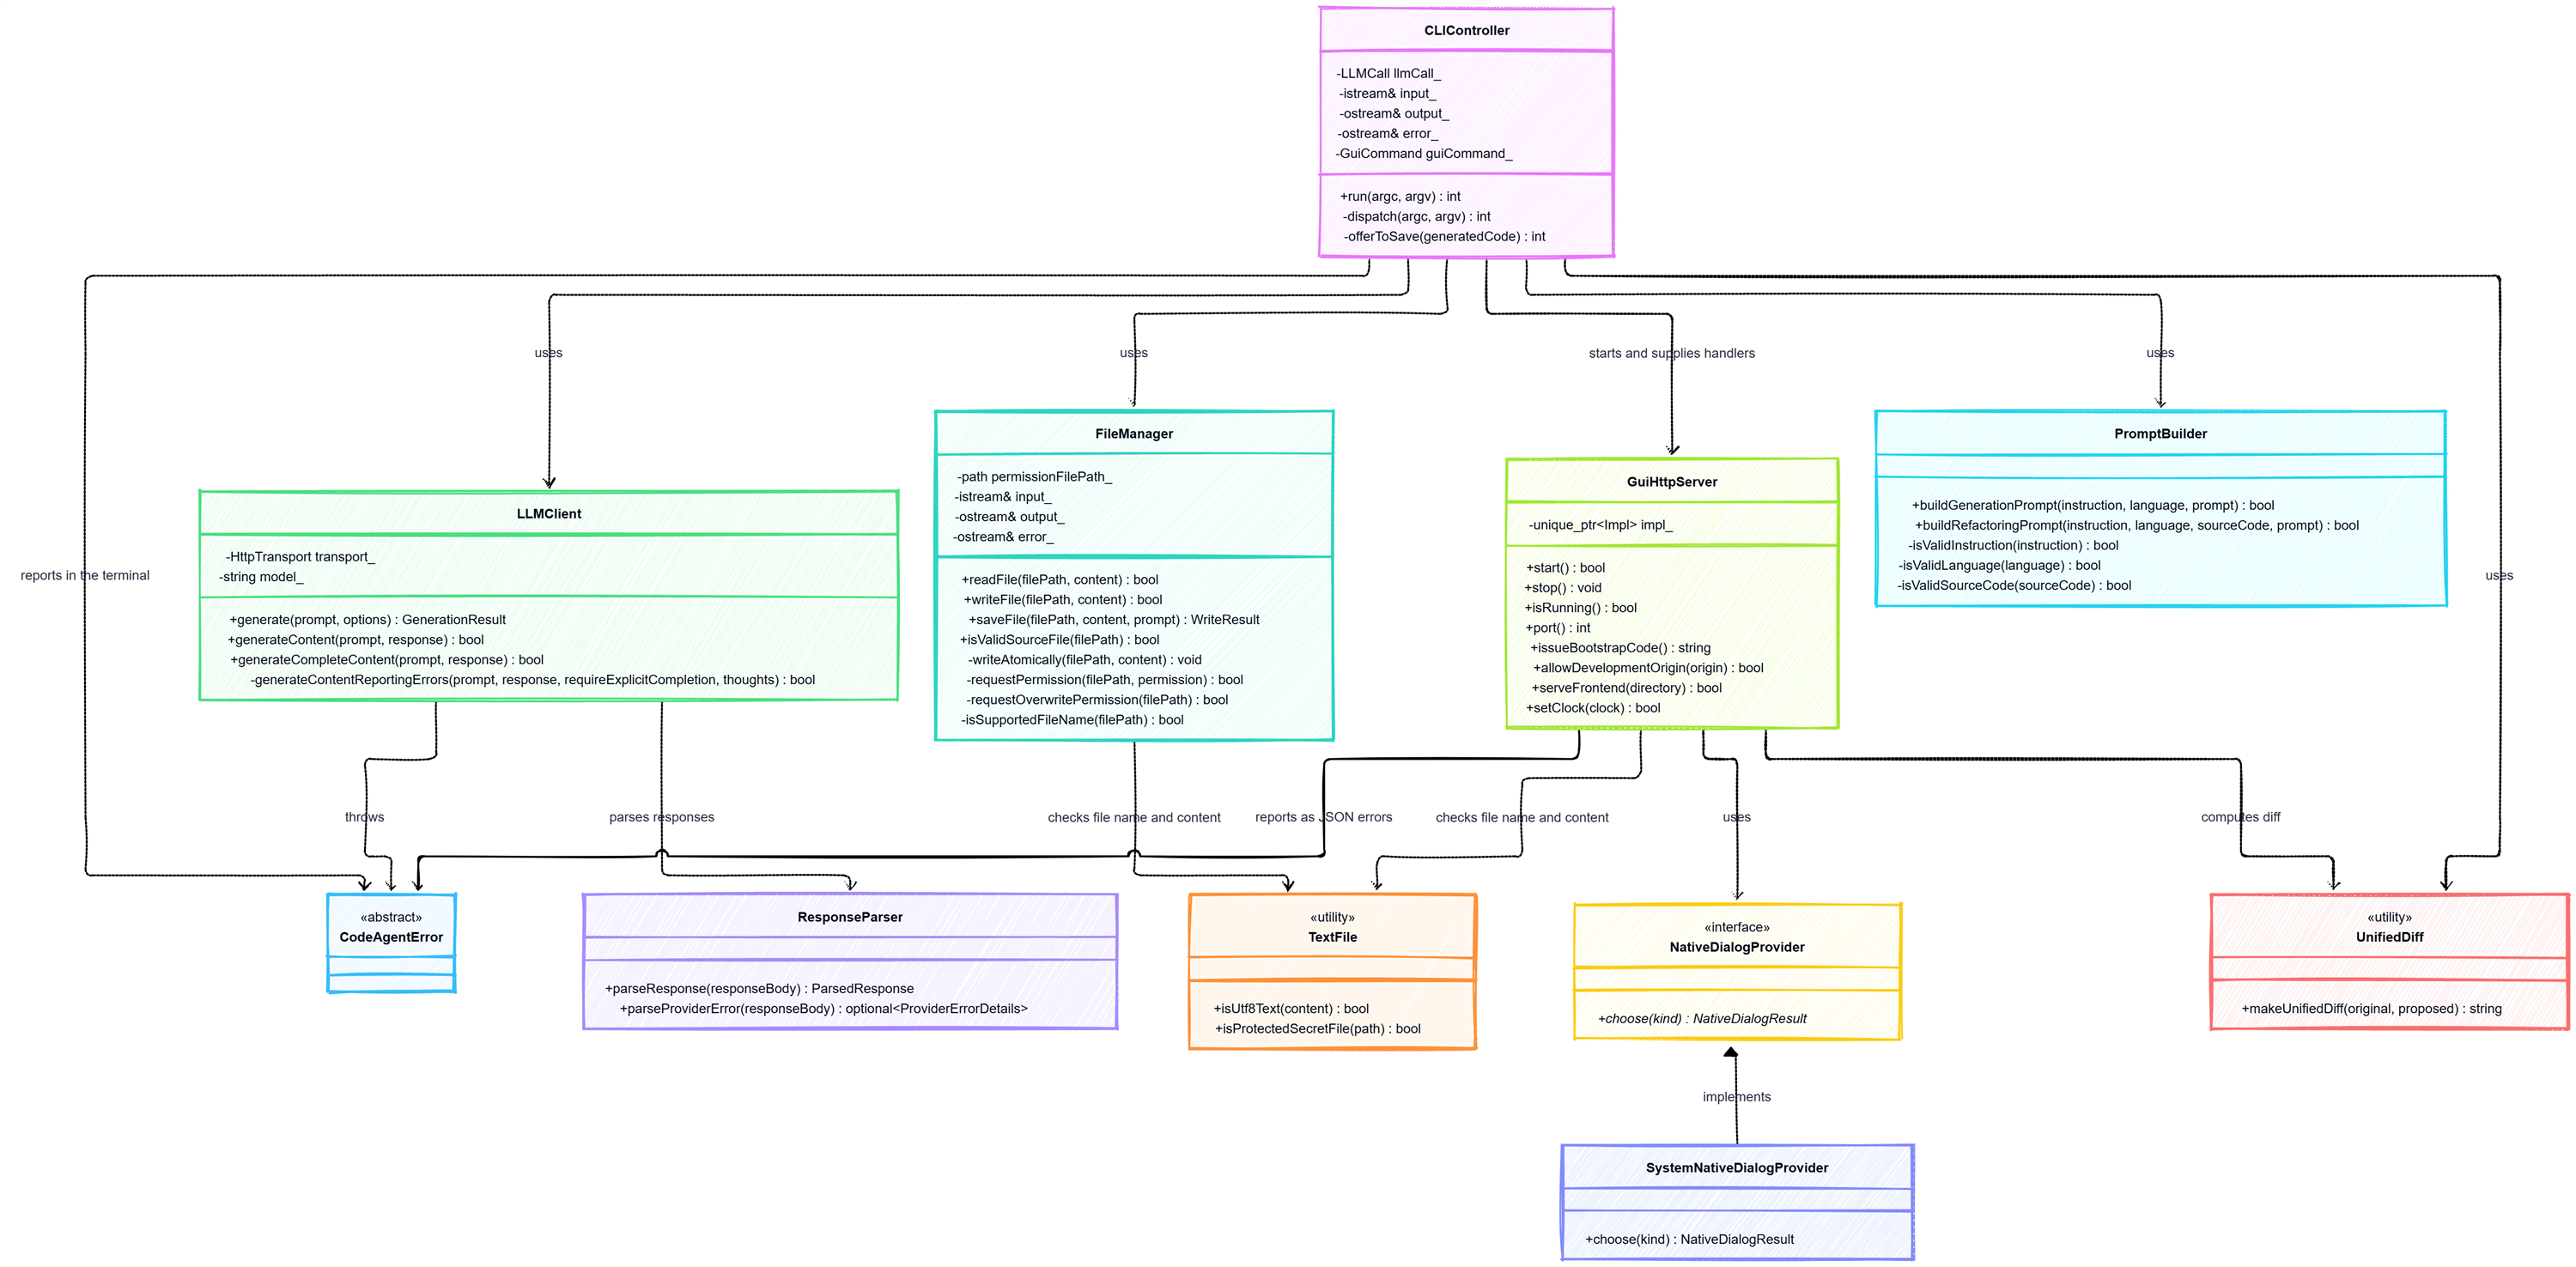
\includegraphics[width=\dimexpr\paperwidth-1.5cm\relax]{screenshots/uml-class.png}}}%
  {\codeagentShot{screenshots/uml-class.png}{Class diagram, view 1}}
\caption{UML class diagram, view 1: application classes and their dependencies}
\label{fig:ca-uml-class}
\end{figure}

\begin{figure}[htbp]
\centering
\codeagentShot{screenshots/uml-errors.png}{Class diagram, view 2}
\caption{UML class diagram, view 2: the \texttt{CodeAgentError} exception hierarchy}
\label{fig:ca-uml-errors}
\end{figure}

\begin{figure}[htbp]
\centering
\codeagentShot{screenshots/uml-seq-cli-generate.png}{CLI code generation sequence}
\caption{UML sequence diagram: CLI code generation with optional save}
\label{fig:ca-uml-seq-gen}
\end{figure}

\begin{figure}[htbp]
\centering
\codeagentShot{screenshots/uml-seq-cli-refactor.png}{CLI refactoring sequence}
\caption{UML sequence diagram: CLI refactoring with diff and approval}
\label{fig:ca-uml-seq-cli}
\end{figure}

\begin{figure}[htbp]
\centering
\codeagentShot{screenshots/uml-seq-gui-refactor.png}{GUI refactoring sequence}
\caption{UML sequence diagram: GUI refactoring proposal lifecycle}
\label{fig:ca-uml-seq-gui}
\end{figure}

\begin{figure}[htbp]
\centering
\codeagentShot[0.42]{screenshots/uml-state.png}{Proposal state diagram}
\caption{UML state diagram: refactoring proposal states}
\label{fig:ca-uml-state}
\end{figure}

% =====================================================================
\section{Advanced C++ Mechanics}
\label{sec:ca-adv}
% =====================================================================

\subsection{Exception Handling (try / throw / catch)}

Errors are \emph{thrown} as typed exceptions at the point of failure and
\emph{caught} at well-defined boundaries:
\begin{itemize}
  \item \texttt{main} (start-up failures);
  \item \texttt{CLIController::\allowbreak{}run} (any command failure becomes a message
    and exit code~1);
  \item each HTTP route handler and the server-wide exception handler (any
    failure becomes a JSON error and the server keeps running).
\end{itemize}

\begin{lstlisting}[style=codeagentcpp,caption={Throwing typed exceptions from HTTP status codes (\texttt{LLMClient.cpp}, abridged)},label={lst:ca-throw}]
[[noreturn]] void throwHttpError(long httpStatus, const std::string& responseBody,
                                 const std::string& model) {
    const auto details = ResponseParser().parseProviderError(responseBody);
    const std::string diagnostic = describeProviderError(httpStatus, details);
    const std::string status = details ? details->status : "";
    const std::string reason = details ? details->reason : "";
    if (httpStatus == 401 || httpStatus == 403 || status == "UNAUTHENTICATED" ||
        status == "PERMISSION_DENIED" || reason == "API_KEY_INVALID") {
        throw AuthenticationError(diagnostic);
    }
    if (httpStatus == 429 || status == "RESOURCE_EXHAUSTED") {
        const bool quotaExhausted = details && hasDailyQuotaViolation(*details);
        throw RateLimitError(quotaExhausted, details ? details->retryDelay : std::nullopt,
                             diagnostic);
    }
    if (httpStatus == 408 || httpStatus == 504 || status == "DEADLINE_EXCEEDED") {
        throw TimeoutError(diagnostic);
    }
    if (httpStatus >= 500) throw ProviderUnavailableError(diagnostic);
    // ... 404 -> ProviderError("model not found"), others -> ProviderError
}
\end{lstlisting}

\begin{lstlisting}[style=codeagentcpp,caption={The CLI error boundary: catch from most specific to most general},label={lst:ca-catch}]
int CLIController::run(int argc, char* argv[]) {
    try {
        return dispatch(argc, argv);
    } catch (const CodeAgentError& failure) {          // all project errors (polymorphic)
        error_ << failure.what() << '\n';
        if (!failure.diagnostic().empty())
            error_ << "Details: " << failure.diagnostic() << '\n';
    } catch (const std::bad_alloc&) {                   // out of memory
        error_ << "Error: CodeAgent ran out of memory. ...\n";
    } catch (const std::exception& failure) {           // anything else, secrets redacted
        error_ << "Error: An unexpected internal error occurred ("
               << redactSecrets(failure.what()) << "). Please retry.\n";
    }
    return 1;
}
\end{lstlisting}

Advanced exception techniques used:
\begin{itemize}
  \item \texttt{[[noreturn]]} functions such as \texttt{throwHttpError} and
    \texttt{throwFileSystemError}, which maps \texttt{std::\allowbreak{}error\_code}
    values to the right subclass.
  \item \texttt{noexcept} on getters and logging functions.
  \item \texttt{std::\allowbreak{}exception\_ptr} with \texttt{std::\allowbreak{}current\_exception} and
    \texttt{std::\allowbreak{}rethrow\_exception} in \texttt{logUnexpectedException} and
    the server's exception handler.
  \item \textbf{Exception-safe copies}: exception members are stored as
    \texttt{std::\allowbreak{}shared\_ptr<const T>}, because copying an exception during
    throw must not itself throw.
  \item \textbf{Secret redaction at construction}: every diagnostic passes
    through \texttt{redactSecrets}, so no catch site can leak the API key.
\end{itemize}

\subsection{Memory and Resource Management (RAII and Smart Pointers)}

The code base contains \textbf{no raw \texttt{new} or \texttt{delete}}. Every
resource is owned by an object whose destructor releases it. C++ guarantees
that destructors run on every exit path, including exceptions.

\begin{table}[htbp]
\centering\small
\begin{tabular}{|p{5.4cm}|p{4.4cm}|p{4.2cm}|}
\hline
\textbf{RAII owner} & \textbf{Resource} & \textbf{Location} \\ \hline
\texttt{std::\allowbreak{}unique\_ptr<CURL, CurlEasyDeleter>} & libcurl request handle & \texttt{LLMClient.cpp} \\ \hline
\texttt{std::\allowbreak{}unique\_ptr<curl\_slist, CurlHeaderListDeleter>} & libcurl header list & \texttt{LLMClient.cpp} \\ \hline
\texttt{TemporaryFileGuard} & temporary file on disk & \texttt{FileManager.cpp} \\ \hline
\texttt{FileDescriptor} & POSIX file descriptor & \texttt{GuiHttpServer.cpp} \\ \hline
\texttt{ProposalCapacityReservation} & reserved proposal slot & \texttt{GuiHttpServer.cpp} \\ \hline
\texttt{std::\allowbreak{}lock\_guard<std::\allowbreak{}mutex>} & mutex lock & \texttt{GuiHttpServer.cpp} \\ \hline
\texttt{std::\allowbreak{}unique\_ptr<Impl>} + destructor calling \texttt{stop()} & server socket and listener thread & \texttt{GuiHttpServer.cpp} \\ \hline
\texttt{std::\allowbreak{}shared\_ptr<NativeDialogProvider>} & shared dialog provider & \texttt{GuiHttpServer.hpp} \\ \hline
\end{tabular}
\caption{RAII and smart-pointer ownership}
\label{tab:ca-raii}
\end{table}

\begin{lstlisting}[style=codeagentcpp,caption={A scope guard: the temporary file is removed on any failure path},label={lst:ca-guard}]
class TemporaryFileGuard {
public:
    explicit TemporaryFileGuard(std::filesystem::path path) : path_(std::move(path)) {}
    ~TemporaryFileGuard() {
        if (!released_) {
            std::error_code ignored;
            std::filesystem::remove(path_, ignored);   // never throws in a destructor
        }
    }
    TemporaryFileGuard(const TemporaryFileGuard&) = delete;             // non-copyable
    TemporaryFileGuard& operator=(const TemporaryFileGuard&) = delete;
    void release() noexcept { released_ = true; }   // called after a successful rename
private:
    std::filesystem::path path_;
    bool released_ = false;
};
\end{lstlisting}

Further memory-related techniques:
\begin{itemize}
  \item \textbf{Move semantics} (\texttt{std::\allowbreak{}move}) transfer large strings,
    such as generated code and response bodies, without copying.
  \item C++17 \textbf{map node handles} (\texttt{extract}/\texttt{insert})
    swap proposals without allocation, and restore the old entry if
    insertion fails.
  \item \textbf{Bounded buffers}: a 2\,MiB limit on Gemini responses, a
    1\,MiB limit on HTTP requests, 512\,KiB editor files, 128 proposals and
    256 remembered documents.
\end{itemize}

\subsection{Templates and Generic Programming}

The project relies heavily on C++ templates through the standard library and
its dependencies, choosing template arguments to model ownership and policy:
\begin{itemize}
  \item \textbf{Class templates with a policy parameter:}
    \texttt{std::\allowbreak{}unique\_ptr<CURL, CurlEasyDeleter>} combines the generic
    smart pointer with a custom deleter type, so one template manages a C
    resource.
  \item \textbf{Type-erasing class template:}
    \texttt{std::\allowbreak{}function<bool(const std::\allowbreak{}string\&, ...)>} stores any callable
    (function, lambda, functor). It is used for \texttt{HttpTransport},
    \texttt{LLMCall}, \texttt{GenerationHandler}, \texttt{RefactoringHandler}
    and \texttt{Clock}.
  \item \textbf{Vocabulary templates:}
    \texttt{std::\allowbreak{}optional<std::\allowbreak{}string>} (an optional finish reason),
    \texttt{std::\allowbreak{}optional<ProviderErrorDetails>},
    \texttt{std::\allowbreak{}shared\_ptr<const T>}, and \texttt{std::\allowbreak{}atomic<int>}.
  \item \textbf{Container templates:} \texttt{std::\allowbreak{}map}, \texttt{std::\allowbreak{}list},
    \texttt{std::\allowbreak{}vector}, \texttt{std::\allowbreak{}unordered\_set}, \texttt{std::\allowbreak{}pair}
    and \texttt{std::\allowbreak{}tuple}. Tuples give lexicographic ordering for proposal
    eviction.
  \item \textbf{Function templates:} \texttt{std::\allowbreak{}make\_unique<Impl>},
    \texttt{std::\allowbreak{}make\_shared<const std::\allowbreak{}string>}, and nlohmann/json's
    \texttt{body["x"].get<std::\allowbreak{}string>()}. Generic algorithms
    (\texttt{std::\allowbreak{}transform}, \texttt{std::\allowbreak{}all\_of}, \texttt{std::\allowbreak{}remove\_if})
    are parameterised with lambdas.
\end{itemize}

\subsection{Operator Overloading}

\begin{itemize}
  \item \textbf{Function-call operator} \texttt{operator()} is overloaded to
    create function objects (functors) that act as custom deleters:
\begin{lstlisting}[style=codeagentcpp,caption={Overloaded \texttt{operator()} used as a smart-pointer deleter},label={lst:ca-functor}]
struct CurlEasyDeleter {
    void operator()(CURL* handle) const noexcept { curl_easy_cleanup(handle); }
};
struct CurlHeaderListDeleter {
    void operator()(curl_slist* list) const noexcept { curl_slist_free_all(list); }
};
using CurlHandle     = std::unique_ptr<CURL, CurlEasyDeleter>;
using CurlHeaderList = std::unique_ptr<curl_slist, CurlHeaderListDeleter>;
\end{lstlisting}
  \item \textbf{Deleted assignment operators}
    (\texttt{operator=(const T\&) = delete}) on \texttt{GuiHttpServer},
    \texttt{TemporaryFileGuard}, \texttt{FileDescriptor} and
    \texttt{ProposalCapacityReservation}. They prevent two objects from owning
    one socket, file or slot.
  \item Use of library-overloaded operators: stream insertion
    \texttt{operator<{}<} for all terminal output, \texttt{std::\allowbreak{}string}
    \texttt{operator+}, \texttt{nlohmann::\allowbreak{}json::\allowbreak{}operator[]}, and the
    \texttt{operator bool} of \texttt{std::\allowbreak{}function} and
    \texttt{std::\allowbreak{}optional}.
\end{itemize}

\subsection{Concurrency}
\begin{itemize}
  \item The GUI server answers requests on a worker-thread pool. Shared state
    is protected by separate mutexes: \texttt{configMutex\_},
    \texttt{proposalMutex\_}, \texttt{saveMutex\_}, \texttt{documentsMutex\_},
    \texttt{sessionMutex\_} and \texttt{lifecycleMutex\_}.
  \item \texttt{std::\allowbreak{}call\_once} initialises libcurl exactly once, and a
    function-local \texttt{static} loads the \texttt{.env} files once,
    thread-safely.
  \item Ctrl+C is handled with a \texttt{volatile std::\allowbreak{}sig\_atomic\_t} flag,
    the only async-signal-safe way to communicate with the main loop.
  \item Tests prove correctness under contention:
    \texttt{ConcurrentApprovalAndRejectionHaveOneWinner} and
    \texttt{ConcurrentRefactorsCannotOverbookLastCapacitySlot}.
\end{itemize}

\subsection{Other Modern C++ Features}
C++17 \texttt{std::\allowbreak{}filesystem} (\texttt{canonical}, \texttt{symlink\_status},
\texttt{lexically\_normal}), \texttt{std::\allowbreak{}chrono::\allowbreak{}steady\_clock} timeouts,
\texttt{enum class} for every closed set of outcomes, \texttt{constexpr}
constants, delegating and \texttt{explicit} constructors, \texttt{override}
and \texttt{final}, raw string literals, if-with-initialiser, lambdas with
explicit captures, and type aliases (\texttt{using}).

% =====================================================================
\section{Frontend and Backend Integration}
\label{sec:ca-integration}
% =====================================================================

\subsection{Separation of Concerns}
\begin{itemize}
  \item \textbf{Backend (C++)} holds all business logic: prompts, Gemini
    calls, response validation, diffs, proposal state, file I/O and
    security.
  \item \textbf{CLI frontend (C++)}: \texttt{CLIController} handles only
    argument parsing and terminal interaction.
  \item \textbf{GUI frontend (JavaScript)} holds only user-interface state:
    \begin{itemize}
      \item \texttt{api.js} is the single module that performs HTTP requests
        and validates every response;
      \item \texttt{proposalWorkflow.js} is the client-side review state
        machine;
      \item \texttt{diffView.js} renders diffs safely with
        \texttt{textContent};
      \item \texttt{app.js} wires the user interface together.
    \end{itemize}
  \item \textbf{Shared core:} both front ends use the same
    \texttt{PromptBuilder}, \texttt{LLMClient} and \texttt{ResponseParser}.
    The GUI reaches them through handler lambdas defined in
    \texttt{CLIController.cpp}, so the Gemini integration is never
    duplicated.
\end{itemize}

\subsection{Communication Protocol and Security}

The browser and the C++ server communicate with JSON over HTTP on
\texttt{127.0.0.1}. Start-up uses a one-time handshake:
\begin{enumerate}
  \item \texttt{codeagent gui} opens
    \texttt{http:/\allowbreak{}/\allowbreak{}127.0.0.1:8080/\allowbreak{}\#bootstrap=<code>}. The URL fragment is
    never sent to servers.
  \item The page sends \texttt{POST /\allowbreak{}api/\allowbreak{}session \{"bootstrap": code\}}. The
    server checks the single-use code (valid for 5 minutes, compared in
    constant time) and returns a 256-bit session token, plus an
    \texttt{HttpOnly; SameSite=Strict} cookie for page reloads.
  \item Every later request carries \texttt{X-CodeAgent-Token}. Before any
    route runs, a pre-routing handler verifies the Host header (against DNS
    rebinding), the Origin header (against other websites) and the token.
\end{enumerate}

\begin{lstlisting}[style=codeagentplain,caption={The single HTTP function of the frontend (\texttt{frontend/js/api.js}, abridged)},label={lst:ca-fetch}]
async function requestJson(path, { method = 'GET', body, session = false } = {}) {
  const options = { method, headers: { Accept: 'application/json' } };
  if (session) options.credentials = 'include';
  else if (sessionToken !== null) options.headers['X-CodeAgent-Token'] = sessionToken;
  if (body !== undefined) {
    options.headers['Content-Type'] = 'application/json';
    options.body = JSON.stringify(body);
  }
  const response = await fetchImpl(`${normalizedBaseUrl}${path}`, options);
  const payload = JSON.parse(await response.text());
  if (!response.ok) {
    const code = payload?.error?.code ?? 'HTTP_ERROR';
    if (code === 'UNAUTHORIZED') sessionToken = null;
    throw new ApiError(code, payload?.error?.message, response.status);
  }
  return payload;
}
\end{lstlisting}

\subsection{HTTP API}

\begin{table}[htbp]
\centering\scriptsize
\begin{tabular}{|p{4.6cm}|p{4.6cm}|p{4.6cm}|}
\hline
\textbf{Endpoint} & \textbf{Purpose} & \textbf{Side effect} \\ \hline
\texttt{POST /\allowbreak{}api/\allowbreak{}session} & exchange bootstrap code or cookie for the token & consumes the code \\ \hline
\texttt{GET /\allowbreak{}api/\allowbreak{}health}, \texttt{GET /\allowbreak{}api/\allowbreak{}config} & status and directories & none \\ \hline
\texttt{POST /\allowbreak{}api/\allowbreak{}generate} & generate code & calls Gemini \\ \hline
\texttt{POST /\allowbreak{}api/\allowbreak{}refactor} & create a refactoring proposal & calls Gemini; proposal \texttt{PENDING} \\ \hline
\texttt{POST /\allowbreak{}api/\allowbreak{}diff} & unified diff of a proposal or two buffers & none \\ \hline
\texttt{POST /\allowbreak{}api/\allowbreak{}changes/\allowbreak{}\{id\}/\allowbreak{}approve} & approve a proposal (does \emph{not} save) & \texttt{PENDING} $\rightarrow$ \texttt{APPROVED} \\ \hline
\texttt{POST /\allowbreak{}api/\allowbreak{}changes/\allowbreak{}\{id\}/\allowbreak{}reject} & reject a proposal & \texttt{PENDING} $\rightarrow$ \texttt{REJECTED} \\ \hline
\texttt{POST /\allowbreak{}api/\allowbreak{}changes/\allowbreak{}\{id\}/\allowbreak{}mark-applied} & proposal applied in the editor & \texttt{APPROVED} $\rightarrow$ \texttt{APPLIED} \\ \hline
\texttt{POST /\allowbreak{}api/\allowbreak{}files/\allowbreak{}open-dialog} & native file picker & starts a child process \\ \hline
\texttt{POST /\allowbreak{}api/\allowbreak{}files/\allowbreak{}read} & open a file in the editor & reads a file \\ \hline
\texttt{POST /\allowbreak{}api/\allowbreak{}files/\allowbreak{}write} & save an opened file in place (conflict detection) & writes a file atomically \\ \hline
\texttt{POST /\allowbreak{}api/\allowbreak{}output/\allowbreak{}select-directory} & choose the output directory & session state \\ \hline
\texttt{POST /\allowbreak{}api/\allowbreak{}save} & Save As / save an approved proposal & writes a new file \\ \hline
\end{tabular}
\caption{HTTP API implemented by \texttt{GuiHttpServer}}
\label{tab:ca-api}
\end{table}

Every route checks the content type, validates the \emph{exact} JSON shape
(unknown fields such as \texttt{apiKey} are rejected), and reports errors in a
single format: \texttt{\{"error":\{"code":...,\allowbreak{}"message":...\}\}}.

\subsection{Persistent Storage and File I/O}
\label{sec:ca-storage}

\begin{itemize}
  \item \textbf{Source files (read):}
    \begin{itemize}
      \item binary-mode reads that keep CRLF line endings;
      \item strict UTF-8 validation;
      \item in the GUI, a 512\,KiB limit enforced while reading;
      \item FIFOs and devices are refused without blocking
        (\texttt{O\_NONBLOCK} + \texttt{fstat}).
    \end{itemize}
  \item \textbf{Source files (write):}
    \begin{itemize}
      \item atomic replacement through a temporary file and
        \texttt{rename};
      \item the GUI writer also uses \texttt{O\_EXCL} temporary files,
        \texttt{fsync}, preservation of permission bits, and
        \texttt{link()} for new files, so a file created concurrently is
        never overwritten;
      \item symbolic-link targets are refused.
    \end{itemize}
  \item \textbf{Change detection:} an FNV-1a 64-bit revision hash returned on
    open. Saving over a file modified externally (for example in VS Code)
    requires explicit confirmation (\texttt{409 FILE\_CHANGED\_ON\_DISK}).
  \item \textbf{Persistent permission store:} answering \emph{[A] Always
    allow} at a CLI permission prompt appends \texttt{read|path} or
    \texttt{write|path} to \texttt{.codeagent/\allowbreak{}permissions.txt}. Later runs
    read this file and skip the question. Overwriting still always asks.
  \item \textbf{Configuration storage:} \texttt{.env} files are read in
    priority order: \texttt{\$CODEAGENT\_ENV\_FILE}, then \texttt{./\allowbreak{}.env},
    then \texttt{\textasciitilde/\allowbreak{}.config/\allowbreak{}codeagent/\allowbreak{}.env}. Variables already
    in the environment are never overwritten.
\end{itemize}

\subsection{Gemini Integration}
\begin{enumerate}
  \item \texttt{LLMClient::\allowbreak{}generate} reads \texttt{GEMINI\_API\_KEY}. If it
    is missing, a \texttt{ConfigurationError} is thrown before any network
    access.
  \item It builds the JSON body
    \texttt{\{"contents":[\{"parts":[\{"text": prompt\}]\}]\}}.
  \item It POSTs to
    \texttt{https:/\allowbreak{}/\allowbreak{}generativelanguage.googleapis.com/\allowbreak{}v1beta/\allowbreak{}models/\allowbreak{}gemini-3.5-flash:generateContent}
    through libcurl:
    \begin{itemize}
      \item the key is sent in the \texttt{x-goog-api-key} header, never in
        the URL;
      \item TLS certificates are verified;
      \item timeouts are 10\,s to connect and 60\,s in total.
    \end{itemize}
  \item \texttt{ResponseParser} validates every level of the reply. Unknown
    finish reasons are treated as failures (fail-closed). A refactoring must
    end with \texttt{finishReason = STOP}, so truncated code is never offered
    for saving.
\end{enumerate}

% =====================================================================
\section{Testing and Quality Assurance}
\label{sec:ca-testing}
% =====================================================================

All tests run offline, using the dependency-injection seams described in
Section~\ref{sec:ca-oop}. GoogleTest cases are registered individually with
CTest through \texttt{gtest\_discover\_tests}.

\begin{table}[htbp]
\centering\small
\begin{tabular}{|p{4.7cm}|r|p{7.6cm}|}
\hline
\textbf{Test file} & \textbf{Cases} & \textbf{What is verified} \\ \hline
\texttt{FileManagerTest.cpp} & 15 & any extension, \texttt{.env} refusal, CRLF round-trip, overwrite confirmation, permission errors \\ \hline
\texttt{PromptBuilderTest.cpp} & 9 & templates, empty-input rejection, determinism \\ \hline
\texttt{LLMClientTest.cpp} & 26 & HTTP errors, timeouts, quota, malformed JSON, 2\,MiB limit, key never in errors \\ \hline
\texttt{ResponseParserTest.cpp} & 32 & JSON structure, finish reasons, thoughts, fence stripping \\ \hline
\texttt{UnifiedDiffTest.cpp} & 7 & diff correctness, line endings \\ \hline
\texttt{EnvLoaderTest.cpp} & 8 & \texttt{.env} parsing and priority \\ \hline
\texttt{CLIControllerTest.cpp} & 26 & approval-gated writes, rejection, invalid input, save prompts \\ \hline
\texttt{CodeAgentErrorTest.cpp} & 7 & hierarchy, codes, redaction \\ \hline
\texttt{GuiHttpServerTest.cpp} & 84 & real HTTP: authentication, Host/Origin, every endpoint, proposal states, concurrency, conflicts, permissions \\ \hline
\textbf{C++ total} & \textbf{214} & \texttt{ctest -{}-test-dir build -{}-output-on-failure} \\ \hline
\texttt{frontend/\allowbreak{}tests/\allowbreak{}*.test.mjs} & 79 & API validation, workflow gating, diff rendering, real \texttt{app.js} on a test DOM \\ \hline
\end{tabular}
\caption{Automated test suites}
\label{tab:ca-tests}
\end{table}

The full suite passed in our verification run: 214/214 C++ tests (run with
\texttt{ctest -j1}) and 79/79 frontend tests. The FileManager tests share one
sandbox directory, so the suite is currently run serially. Giving each test
its own directory is listed as future work.

\begin{figure}[htbp]
\centering
\codeagentShot{screenshots/tests-ctest.png}{Terminal: \texttt{ctest -{}-test-dir build -{}-output-on-failure} showing 100\% tests passed}
\caption{C++ test results: \texttt{scripts/\allowbreak{}install.sh} runs all 214 CTest tests (100\% passed) before installing \texttt{codeagent}}
\label{fig:ca-ctest}
\end{figure}

\begin{figure}[htbp]
\centering
\codeagentShot{screenshots/tests-node.png}{Terminal: \texttt{node -{}-test frontend/\allowbreak{}tests/\allowbreak{}*.test.mjs} showing 79 passing}
\caption{Frontend test results (Node.js)}
\label{fig:ca-node}
\end{figure}

% =====================================================================
\section{Build System}
% =====================================================================

CMake 3.15+ builds the project with C++17 (\texttt{CMAKE\_CXX\_STANDARD 17},
extensions off) and warnings (\texttt{-Wall -Wextra -Wpedantic}).
\begin{itemize}
  \item libcurl and nlohmann/json come from the system.
  \item GoogleTest v1.14.0 and cpp-httplib v0.58.0 are fetched at pinned
    versions with \texttt{FetchContent}.
  \item Static libraries: \texttt{CodeAgentError}, \texttt{UnifiedDiff},
    \texttt{GuiHttpServer}.
  \item The \texttt{codeagent} executable links them.
  \item \texttt{install()} rules and \texttt{scripts/\allowbreak{}install.sh} install the
    binary and frontend to \texttt{\textasciitilde/\allowbreak{}.local}, so
    \texttt{codeagent} works from any folder.
\end{itemize}

\begin{lstlisting}[style=codeagentplain,caption={Build, test and run},label={lst:ca-build}]
cmake -S . -B build
cmake --build build
ctest --test-dir build --output-on-failure
node --test frontend/tests/*.test.mjs
export GEMINI_API_KEY=...        # or put it in .env
./build/codeagent help
./build/codeagent generate "a function that checks whether a string is a palindrome"
./build/codeagent refactor src/example.cpp "improve error handling"
./build/codeagent gui
\end{lstlisting}

% =====================================================================
\section{Version Control and Collaboration}
\label{sec:ca-git}
% =====================================================================

The project was developed in Git with feature branches, integration branches
and frequent, small commits that follow the Conventional Commits style
(\texttt{feat(gui):}, \texttt{fix:}, \texttt{docs:}, \texttt{test:},
\texttt{chore:}).

\begin{table}[htbp]
\centering\small
\begin{tabular}{|p{6cm}|p{7.5cm}|}
\hline
\textbf{Metric} & \textbf{Value} \\ \hline
Total commits & 61 (Lalitadithya Kariyam: 30, Samuel John: 31) \\ \hline
Lines added / deleted (non-merge) & Lalitadithya: +9{,}644 / $-$966; Samuel: +13{,}385 / $-$1{,}721 \\ \hline
Branches & \texttt{main}, \texttt{feature/\allowbreak{}gui-backend}, \texttt{feature/\allowbreak{}gui-frontend}, \texttt{feature/\allowbreak{}setup-googletest}, \texttt{integration/\allowbreak{}gui-complete}, \texttt{integration/\allowbreak{}gui-full-app} \\ \hline
Merge commits & \texttt{225ba46} (frontend into backend), \texttt{cb6e3f6}, \texttt{bfa1bad} (integration into \texttt{main}) \\ \hline
Development period & 1 October 2026 -- 29 October 2026 \\ \hline
\end{tabular}
\caption{Repository statistics}
\label{tab:ca-gitstats}
\end{table}

\paragraph{Parallel collaboration.}
On 26--28 October both members committed on the same days (25 commits on
27~October alone). The backend and frontend branches advanced in parallel, and
each backend endpoint was followed by its frontend integration. Examples:
\texttt{c30c7cf} \emph{add GUI code generation endpoint} $\rightarrow$
\texttt{7700d60} \emph{connect code generation to backend}; and
\texttt{42b433b} \emph{add GUI refactoring endpoint} $\rightarrow$
\texttt{3d038e1} \emph{integrate proposal review workflow}. The frontend
branch was merged into the backend branch (\texttt{225ba46}) so the UI was
built against the real API, then integrated into \texttt{main}
(\texttt{bfa1bad}).

\begin{table}[htbp]
\centering\small
\begin{tabular}{|p{2.6cm}|p{5.5cm}|p{5.5cm}|}
\hline
\textbf{Phase} & \textbf{Lalitadithya Kariyam (251130)} & \textbf{Samuel John (251118)} \\ \hline
Foundation (1--13 Oct) & CLI foundation \& command controller (\texttt{a36e672}), \texttt{planning.md} & \texttt{FileManager} (\texttt{61d8e20}), GoogleTest setup (\texttt{6666888}) \\ \hline
Core AI (19--24 Oct) & \texttt{PromptBuilder} (\texttt{74e1533}), Gemini integration (\texttt{137a6be}) & \texttt{ResponseParser} (\texttt{35d584d}), file-safety fixes (\texttt{5fea4c6}, \texttt{a72d40d}) \\ \hline
GUI backend (26--27 Oct) & API contract (\texttt{47789e6}), HTTP server (\texttt{cc7f573}), health/config (\texttt{566250f}), \texttt{gui} command (\texttt{31ee0da}), generation endpoint (\texttt{c30c7cf}), safe saving (\texttt{8fd772a}) & CLI diff \& approval (\texttt{43e5c87}), refactoring endpoint (\texttt{42b433b}), diff/approval workflow (\texttt{700aebe}), native dialogs (\texttt{4616f81}) \\ \hline
GUI frontend (26--28 Oct) & API client (\texttt{270ec51}), backend status (\texttt{3b21ab0}), secure integration (\texttt{6df7b43}), chat with thoughts (\texttt{1f45db5}), Save As UX (\texttt{a319893}) & HTML structure \& CSS (\texttt{b3b1afe}, \texttt{42eca48}), editor workspace (\texttt{9527284}), proposal review UI (\texttt{95ccde4}, \texttt{3d038e1}), frontend serving (\texttt{0eac287}) \\ \hline
Hardening (28--29 Oct) & Integration merge (\texttt{bfa1bad}), UML diagrams, README & Exception hierarchy (\texttt{a077a64}), interactive save (\texttt{dc4a225}), global install (\texttt{62cdde7}), any-extension files (\texttt{522b973}) \\ \hline
\end{tabular}
\caption{Contribution timeline (selected commits)}
\label{tab:ca-contrib}
\end{table}

\clearpage
% =====================================================================
\section{Results}
\label{sec:ca-results}
% =====================================================================

\subsection{Command-Line Interface}

\begin{figure}[htbp]
\centering
\codeagentShot{screenshots/cli-help.png}{codeagent help}
\caption{CLI help output (\texttt{codeagent help})}
\label{fig:ca-cli-help}
\end{figure}

\begin{figure}[htbp]
\centering
\codeagentShot{screenshots/cli-generate.png}{codeagent generate}
\caption{CLI code generation: generated code is displayed, then saved to a user-chosen path}
\label{fig:ca-cli-generate}
\end{figure}

\begin{figure}[htbp]
\centering
\codeagentShot{screenshots/cli-refactor-diff.png}{codeagent refactor}
\caption{CLI refactoring of a non-C++ file (\texttt{source.dat}): read permission, unified diff, approval, write permission and overwrite confirmation}
\label{fig:ca-cli-refactor}
\end{figure}

\begin{figure}[htbp]
\centering
\begin{minipage}[t]{0.49\linewidth}\centering
\codeagentShot{screenshots/cli-generated-file.png}{Saved generated file}\\[2pt]
\small (a) \texttt{text.cpp} saved by \texttt{generate}
\end{minipage}\hfill
\begin{minipage}[t]{0.49\linewidth}\centering
\codeagentShot{screenshots/cli-refactored-file.png}{Refactored file}\\[2pt]
\small (b) \texttt{source.dat} after \texttt{refactor}: commas became tabs
\end{minipage}
\caption{Files written by the CLI, each only after the user's explicit approval}
\label{fig:ca-cli-files}
\end{figure}

\subsection{Browser GUI}

\begin{figure}[htbp]
\centering
\codeagentShot{screenshots/gui-startup-terminal.png}{codeagent gui}
\caption{Starting the GUI backend with \texttt{codeagent gui}}
\label{fig:ca-gui-start}
\end{figure}

\begin{figure}[htbp]
\centering
\codeagentShot{screenshots/gui-generate.png}{GUI generation}
\caption{GUI code generation in Python with the backend connected: the generated output is shown for review and is not saved}
\label{fig:ca-gui-generate}
\end{figure}

\begin{figure}[htbp]
\centering
\codeagentShot{screenshots/gui-generate-accepted.png}{Generated code accepted}
\caption{Generated code accepted into the editor (not saved), with Gemini's thoughts shown in the chat}
\label{fig:ca-gui-generate-accepted}
\end{figure}

\begin{figure}[htbp]
\centering
\codeagentShot{screenshots/gui-refactor-proposal.png}{Refactoring proposal}
\caption{GUI refactoring proposal: original code, proposed code and the coloured unified diff, with Accept and Reject}
\label{fig:ca-gui-proposal}
\end{figure}

\begin{figure}[htbp]
\centering
\codeagentShot{screenshots/gui-accepted.png}{Accepted proposal}
\caption{Approved proposal applied to the editor; the unsaved marker on \texttt{str.c} shows nothing has been written yet}
\label{fig:ca-gui-accepted}
\end{figure}

\clearpage
% =====================================================================
\section{Demonstration Plan}
\label{sec:ca-demo}
% =====================================================================
\begin{enumerate}
  \item \textbf{Build and tests:} \texttt{cmake -{}-build build},
    \texttt{ctest}, \texttt{node -{}-test} (Figures~\ref{fig:ca-ctest}
    and~\ref{fig:ca-node}).
  \item \textbf{CLI generation:} generate a palindrome checker, save it, then
    try to save it to the same name again to show the overwrite
    confirmation.
  \item \textbf{CLI refactoring:} refactor a small file, show the diff, reject
    it (the file is unchanged), run it again and approve.
  \item \textbf{Error handling:} unset the API key to show the configuration
    error and exit code~1.
  \item \textbf{GUI:} \texttt{codeagent gui} $\rightarrow$ open a file by
    path $\rightarrow$ refactor $\rightarrow$ review the diff $\rightarrow$
    accept (the editor changes, the disk does not) $\rightarrow$ edit the
    file in another editor $\rightarrow$ Save shows the conflict
    confirmation.
  \item \textbf{Code walk-through:} \texttt{CodeAgentError} polymorphism,
    \texttt{respondWithError}, RAII guards, the dependency-injection test
    seams, and the pimpl header.
\end{enumerate}

% =====================================================================
\section{Limitations and Future Work}
% =====================================================================
\begin{itemize}
  \item Share the GUI's stronger atomic writer (permission preservation,
    \texttt{fsync}, unique temporary names) with the CLI
    \texttt{FileManager}.
  \item Give each FileManager test its own sandbox directory so the suite can
    run in parallel (\texttt{ctest -j}).
  \item Extract a \texttt{ProposalStore} class from
    \texttt{GuiHttpServer::\allowbreak{}Impl} to reduce its size.
  \item Add a \texttt{-{}-language} option to the CLI \texttt{generate}
    command.
  \item Optionally restrict which paths the GUI may open, beyond the
    \texttt{.env} rule.
  \item Make the Gemini model configurable, add syntax highlighting, and add
    an automated real-browser end-to-end test and CI.
\end{itemize}

% =====================================================================
\section{Conclusion}
% =====================================================================
CodeAgent meets its requirements:
\begin{itemize}
  \item it generates and refactors code with Gemini from both a CLI and a
    browser GUI (R1, R2, R7);
  \item it never changes a file without an explicit, separate save decision
    (R3, R4);
  \item it keeps the API key out of URLs, logs and the browser (R5);
  \item it turns every failure into a typed, actionable message (R6);
  \item it is verified by 293 automated tests that run offline (R8).
\end{itemize}

The architecture demonstrates object-oriented design in practice: small
encapsulated classes, an abstract exception hierarchy with virtual functions,
interface-based polymorphism, composition, and dependency injection. On the
advanced C++ side it uses RAII and smart pointers, exceptions, templates,
functors, concurrency and C++17 features. The Git history shows incremental
and parallel work by both members.

% Restore the float placement used by the rest of the book.
\let\topfraction\codeagentOldTopfraction
\let\bottomfraction\codeagentOldBottomfraction
\let\textfraction\codeagentOldTextfraction
\let\floatpagefraction\codeagentOldFloatpagefraction
\setcounter{topnumber}{\codeagentOldTopnumber}
\setcounter{totalnumber}{\codeagentOldTotalnumber}

\end{document}
